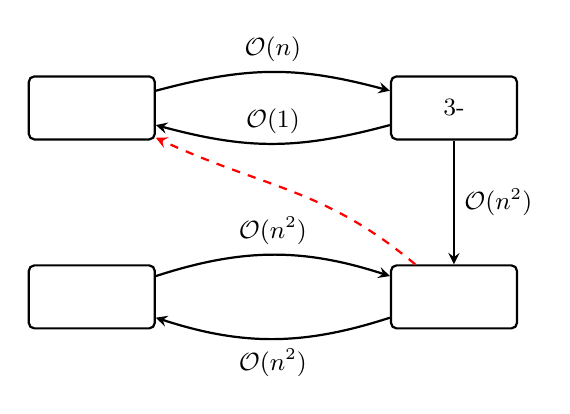
\begin{tikzpicture}[
    >=stealth,
    thick,
    font=\small,
    problem/.style={
        draw,
        rounded corners=2pt,
        minimum width=16mm,
        minimum height=8mm,
        inner sep=2pt,
        align=center
    },
    reduction/.style={->, thick},
    hinted/.style={->, thick, dashed}
]

    % uzly
    \node[problem] (sat)      at (0,2.4) {$\SAT$};
    \node[problem] (threesat) at (4.6,2.4) {$3$-$\SAT$};
    \node[problem] (clique)   at (0,0) {$\KLIKA$};
    \node[problem] (indset)   at (4.6,0) {$\NZMNA$};

    % SAT -> 3-SAT
    \draw[reduction]
        (sat) to[out=15, in=165, looseness=1.05] node[midway, above] {$\mathcal{O}(n)$} (threesat);
    
    % 3-SAT -> SAT
    \draw[reduction]
        (threesat) to[out=-165, in=-15, looseness=1.05] node[midway, above] {$\mathcal{O}(1)$} (sat);

    % 3-SAT -> NzMna
    \draw[reduction]
        (threesat) -- node[midway, right] {$\mathcal{O}(n^2)$} (indset);

    % Klika <-> NzMna
    \draw[reduction, bend left=18]
        (clique) to node[midway, above] {$\mathcal{O}(n^2)$} (indset);

    \draw[reduction, bend left=18]
        (indset) to node[midway, below] {$\mathcal{O}(n^2)$} (clique);

    % NzMna -> SAT (jen naznak)
    \draw[hinted,color=red]
        (indset) to[out=140, in=-25, looseness=1.05] (sat);

\end{tikzpicture}